\documentclass[a4paper, 12pt]{article}

\usepackage{tikz}
\usetikzlibrary{automata}
\usetikzlibrary{positioning}

\title{Task 1}
\author{}
\date{}

\begin{document}
\maketitle

\begin{figure}[h]
  \centering
  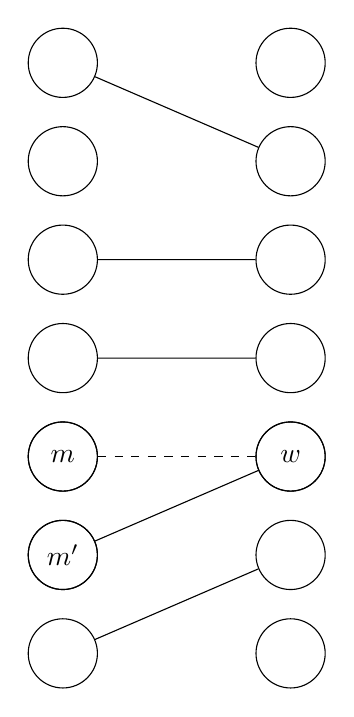
\begin{tikzpicture}[
    node distance=1.25cm,
    every node/.style={
      circle,
      draw
    }
    ]
    \node[state] (1_l) {};
    \foreach \x/\y in {2/1,3/2,4/3,5/4,6/5,7/6}{
      \node[state] (\x_l) [below of=\y_l] {};
    }
    \node[state] (1_r) [right=2cm of 1_l] {};
    \foreach \x/\y in {2/1,3/2,4/3,5/4,6/5,7/6}{
      \node[state] (\x_r) [below of=\y_r] {};
    }
    \node[state] (m) at (5_l) {$m$};
    \node[state] (m') at (6_l) {$m'$};
    \node[state] (w) at (5_r) {$w$};

    \draw
    (1_l) -- (2_r)
    (3_l) -- (3_r)
    (4_l) -- (4_r)
    (m')  -- (w)
    (7_l) -- (6_r)
    ;
    \draw[dashed] (m) -- (w);
  \end{tikzpicture}
\end{figure}


\end{document}
